\chapter{Security} 
\label{ch:security}

\lhead{Chapter 6. \emph{Security}}

In this chapter we will discuss the security in our implementation of NIPEN.
We will also talk about what type of security would be expected in a final implementation of NIPEN. 
There will also be a short mention of HIPAA and what role that act will play in a system like this.
At the end of this chapter we will discuss how to grant third party applications limited access to our system.

\section{Security in our solution}
We cleared it with the customer early that to make it easy and achievable for us to make this proof of concept we had to skip most of the security needed.
Therefore the data used is not encrypted. 
We are only using Hypertext Transfer Protocol (HTTP) for transportation of data and not using the Secure Socket Layer (SSL).  
We have also not implemented an authentication system.
Since we have not implemented an authentication system there is only one user of the system.
Every user of the system has access to that users data.

\section{Security in NIPEN}

In this section we will discuss some of the factors that should be considered when implementing NIPEN on a large scale.
We will briefly cover HIPAA and the different forms of security needed for this type of system like authentication, storage and transportation of the data.


\subsection{HIPAA - Health Insurance Portability and Accountability Act}

After discussing security with the customer we brought up the topic of HIPAA \cite{HIPAA}. 
Even though there is no similar act in Norway the customer believed that taking a starting point from HIPAA to discuss the security in NIPEN would be a smart basis. 

\subsection{Storage of data}
When the data is at rest the network should be protected from intrusions.
The hard drives where the data is stored must be encrypted. \cite{Encryption}
HIPAA does not specify what type of encryption should be used, they only specify that it should be encrypted.

\begin{figure}[H]
\centering
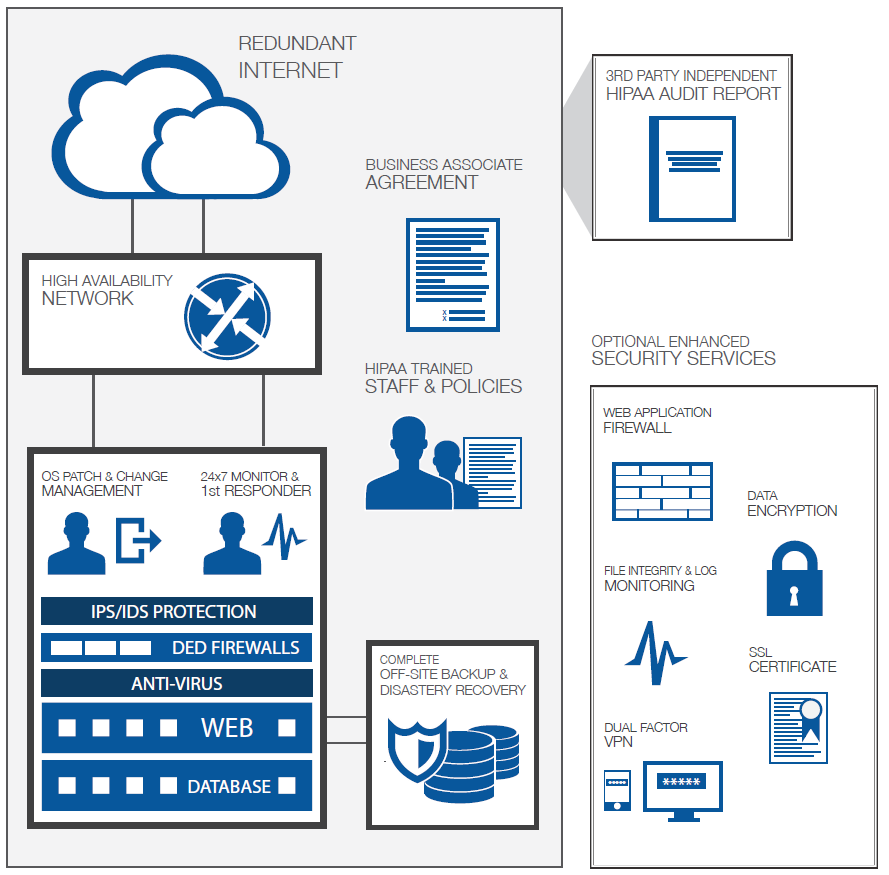
\includegraphics[scale=0.50]{../Figures/hipaa.png}
\caption{HIPAA Compliant Data Center Architecture from www.onlinetech.com}
\label{figure:HIPAA}
\end{figure}

\subsection{Transportation of data}
In HIPAA the transportation of data is described that it needs to use Secure Socket Layer. 
This layer is designed to give communication security over the Internet. \cite{SSL}

\subsection{Authentication}
There are multiple systems already in use today in Norway for authenticating users. 
Some of the biggest systems are MinId, BankID, Buypass and Commfides.
The most widespread right now is BankId, with almost 3 million users as of this writing (\href{https://www.bankid.no/}{https://www.bankid.no/}).
It would be worth a consideration to use BankID to authenticate the citizens. 
The reason behind this is that it is a widespread system and something the citizens are familiar with. 

When considering what type of authentication the medical professionals should use there are multiple factors to consider. 
Ease of use, efficiency and be able to make an audit trail are some extra factors too consider.
It might be as successful to develop a separate system of authenticating the health professionals if BankID turns out to be cumbersome and unable to be used in the different situations needed for this system. 
For HIPAA there needs to be a system to know which information was accessed, when, and by whom. \cite{Audit}

\subsection{Giving data to third party systems}
Not only should this system accept data from third parties. 
There should also be functionality for exporting data from the system to third party providers. 
For this to happen there needs to be a system for the end users, the citizens, to understand where and to whom the data is going.
Any data that is Protected Health Information \cite{PHI}, which is defined as any data classified as health information connected by the patients identifiers, the end user must control how this information is shared. 
In the end its up to the user who they want to share their data with.
What could be smart is to introduce a Norwegian certification so that the end user knows that the data providers they want to export their data to follows the rules mentioned in previous subsections. 
That way it is easier for the user to trust new systems with their sensitive data.

\section{OAuth 2.0}

OAuth 2.0 is a protocol that could potentially be used for our integration platform.
OAuth 1.0 is outdated, and hence we will mainly focus on OAuth 2.0 in this section.
What this protocol does is that it grants third party applications partial access to a system.
In our case this could for example be only access to the API concerning heart rates or weights in NIPEN.

\subsection{What is OAuth?}

Many applications want to have access to an API provider to gain access to a users information.
However, the user doesn't always want to give his/hers credentials to these applications.
Lets say that a user wants to have an application that is able to upload images to his/hers facebook account.
The user doesn't want to give the application the credentials for facebook.
This would be highly insecure, since once the application has the authentication information of a user it is able to do whatever it wants with the account.
To handle this we need some kind of protocol, this is where OAuth comes in.
With OAuth we are able to give a third party application partial access to a system without handing over the credentials of a user.
This is a token based system, where the application receives a token which grants it access to use some of the systems services.

When a third party app wants to use a system that uses OAuth, it first needs to be registered in that system.
Under registration the system usually wants some basic information about the application.
This might include name of the application, a description, logo and etc.
A redirect URI also needs to be registered.
This URI needs to use TLS, i.e. must begin with \textit{https}.
This address is used to send an authentication token from the system to the application.
After the registration, the application should receive a client ID which is used to identify the application at the system.

Now users should be able to connect the application with theirs account on the system.
The way it works is that through the application they will be sent to a website of the system the application wants to connect with.
There the user will be asked if he/she wants to grant permissions to the application.
If the user agrees, then he/she will be redirected to the applications specified redirect URI with an access token as a parameter.
The application will now use this token to access the system.
When the user doesn't want the application to have access to the system any more, he/she can simply disallow the applications access through the systems website.

An example of how OAuth works is given in figure \ref{figure:oauth-in-a-nutshell}.
In this example we see a website that wants to send images to a users facebook account.
If the user allows the application access through facebook, then facebook will send an access token to the website.
Then \textit{www.ImageToFacebook.com} is able to send images to the users account, where the access token is used for authentication.
The user should be able to disallow the website access at any time on facebooks website. \cite{OAuth}

\begin{figure}[h]
\centering
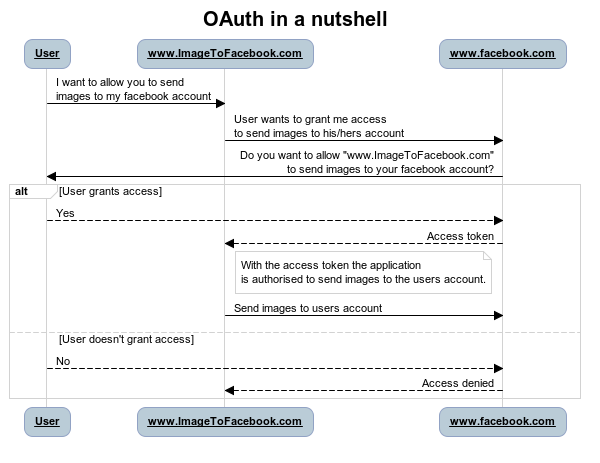
\includegraphics[scale=1.0]{../Figures/oauth-in-a-nutshell.png}
\caption{OAuth in a nutshell}
\label{figure:oauth-in-a-nutshell}
\end{figure}


\subsection{Applying OAuth to NIPEN}

It should not be a problem to apply OAuth to NIPEN.
The functionality that NIPEN needs to implement is a capability of registering third party applications.
Whenever third party applications are registered, they should be associated with a client ID.
This ID should be sent to the third party application.
Users should be able to allow different third party applications limited access to their account.
This could for example be access to only send heart rate measurements (or weights).
When a user allows access to an application an access token should be sent to the specified application, so it gets partial access to the users NIPEN account.
At any time users should be able to remove the applications access to NIPEN.

A summary of how this would work is given in the example below, which illustrates how the granting of permission would work with our heart rate application:

\begin{enumerate}
\item User starts the heart rate application.
\item User wants to grant the application access to push heart rate measurements to NIPEN.
\item User is redirected to the website of NIPEN.
\item User logs in to NIPEN (with e.g. BankID).
\item NIPEN asks the user if he wants to grant the heart rate application access to push heart rate data into NIPEN.
\item If user agrees, an access token is sent to the heart rate application.
\end{enumerate}

With OAuth we should also expand the JSON messages that are sent to NIPEN.
They should now contain a client ID and an access token.
The client ID is used to identify the application that is pushing values to NIPEN, while the access token is used to authorise the application.
A JSON string for a heart rate measurement could now look something like this:

\begin{lstlisting}[language=json]
{
	"clientID": 489431,
	"accessToken": "safDFSAadsffsasdFDSewfaDSFAdsfaewRETrehhgreeErw",
	"userId":453,
	"timestamp":"2013-11-05 12:12:38.0",
	"value":66,
	"unit":"bpm"
}
\end{lstlisting}

This information should be sent in an encrypted format by using https.

NIPEN will now be able to identify what application is sending data, and is also capable of checking if the application is authorised.
The user is also able to grant other applications partial access to his/hers account, without giving these applications their credentials.
Hence, this should be a good way of handling third party applications in NIPEN.

